\begin{name}
	{\tenchude}
	{TOÁN 10}
	{LỚP TOÁN THẦY PHÁT}
	{Thời gian: 90 phút - Không kể thời gian phát đề}
\end{name}
\TN
\Opensolutionfile{ans}[ans/ansBONPA-0D1-OnChuong-De1]
\begin{ex}%[Pj31--2-Đề KT Theo Bài--TeamTeXHoa--Phan Anh]%[0D1N1-2]
	Trong các mệnh đề sau, mệnh đề nào \textbf{sai}?
	\choice
	{\True $-\pi<-2\Leftrightarrow\pi^2<4$}
	{$\pi<4\Leftrightarrow\pi^2<16$}
	{$\sqrt{23}<5\Rightarrow2\sqrt{23}<2{,}5$}
	{$\sqrt{23}<5\Rightarrow-2\sqrt{23}>-2{,}5$}
	\loigiai{
		Mệnh đề sai là \lq\lq $-\pi<-2\Leftrightarrow\pi^2<4$\rq\rq , vì $-\pi<-2$ là mệnh đề đúng và $\pi^2<4$ là mệnh đề sai.
	}
\end{ex}

\begin{ex}%[Pj31--2-Đề KT Theo Bài--TeamTeXHoa--Phan Anh]%[0D1H2-1]
	Cho tập hợp $A=\{x+1\mid x\in\mathbb{N}, x\le 5\}$. Tập hợp $A$ là
	\choice
	{$A=\{1;2;3;4;5\}$}
	{$A=\{0;1;2;3;4;5;6\}$}
	{$A=\{0;1;2;3;4;5\}$}
	{\True $A=\{1;2;3;4;5;6\}$}
	\loigiai{
		Vì $x\in\mathbb{N}, x\le 5$ nên $x\in\{0;1;2;3;4;5\}\Rightarrow x+1\in\{1;2;3;4;5;6\}$ nên $A=\{1;2;3;4;5;6\}$.
	}
\end{ex}

\begin{ex}%[Pj31--2-Đề KT Theo Bài--TeamTeXHoa--Phan Anh]%[0D1H2-1]
	Cho tập hợp $M=\left\{(x;y)\mid x,y\in\mathbb{R}, x^2+y^2\le0\right\}$. Khi đó tập hợp $M$ có bao nhiêu phần tử?
	\choice
	{$0$}
	{\True $1$}
	{$2$}
	{Vô số}
	\loigiai{
		Vì $x^2\ge0$ và $y^2\ge0$ nên $x^2+y^2\ge0$, $\forall x$, $y\in\mathbb{R}$.\\
		Từ đó ta có $x^2+y^2\le0\Leftrightarrow x=y=0$.\\
		Suy ra tập hợp $M$ có một phần tử duy nhất là $(0;0)$.
	}
\end{ex}

\begin{ex}%[Pj31--2-Đề KT Theo Bài--TeamTeXHoa--Phan Anh]%[0D1N1-4]
	Cho mệnh đề $P\Rightarrow Q\colon$ \lq\lq Nếu $3^2+1$ là số chẵn thì $3$ là số lẻ\rq\rq . Chọn mệnh đề đúng trong các mệnh đề sau
	\choice
	{Mệnh đề $Q\Rightarrow P$ là mệnh đề sai}
	{Cả mệnh đề $P\Rightarrow Q$ và $Q\Rightarrow P$ đều sai}
	{Mệnh đề $P\Rightarrow Q$ là mệnh đề sai}
	{\True Cả mệnh đề $P\Rightarrow Q$ và $Q\Rightarrow P$ đều đúng}
	\loigiai{
		Ta có
		\begin{itemize}
			\item $P\colon$ \lq\lq $3^2+1$ là số chẵn\rq\rq  là mệnh đề đúng.
			\item $Q\colon$ \lq\lq $3$ là số lẻ\rq\rq  là mệnh đề đúng.
		\end{itemize}
		Vậy $P\Rightarrow Q$ và $Q\Rightarrow P$ đều là các mệnh đề đúng.
		}
\end{ex}

\begin{ex}%[Pj31--2-Đề KT Theo Bài--TeamTeXHoa--Phan Anh]%[0D1N1-4]
	Cho mệnh đề $P\colon$ \lq\lq Nếu $a+b<2$ thì một trong hai số $a$ và $b$ nhỏ hơn $1$ \rq\rq . Mệnh đề nào sau đây là một cách phát biểu khác của mệnh đề đã cho?
	\choice
	{\True Điều kiện đủ để một trong hai số $a$ và $b$ nhỏ hơn $1$ là $a+b<2$}
	{Điều kiện cần để một trong hai số $a$ và $b$ nhỏ hơn $1$ là $a+b<2$}
	{Điều kiện đủ để $a+b<2$ là một trong hai số $a$ và $b$ nhỏ hơn $1$}
	{Điều kiện cần và đủ để một trong hai số $a$ và $b$ nhỏ hơn $1$ là $a+b<2$}
	\loigiai{
		Mệnh đề $P\colon$ \lq\lq Nếu $a+b<2$ thì một trong hai số $a$ và $b$ nhỏ hơn $1$\rq\rq  có cách phát biểu khác là \lq\lq Điều kiện đủ để một trong hai số $a$ và $b$ nhỏ hơn $1$ là $a+b<2$\rq\rq .¡
		}
\end{ex}

\begin{ex}%[Pj31--2-Đề KT Theo Bài--TeamTeXHoa--Phan Anh]%[0D1N1-5]
	Mệnh đề nào sau đây là mệnh đề phủ định của mệnh đề \lq\lq Mọi động vật đều di chuyển\rq\rq ?
	\choice
	{Mọi động vật đều không di chuyển}
	{Mọi động vật đều đứng yên}
	{\True Có ít nhất một động vật không di chuyển}
	{Có ít nhất một động vật di chuyển}
	\loigiai{Mệnh đề phủ định của mệnh đề \lq\lq $\forall x\in X,P(x)$\rq\rq  là mệnh đề \lq\lq $\exists x\in X,\overline{P(x)}$\rq\rq .\\
		Do đó mệnh đề phủ định của mệnh đề \lq\lq Mọi động vật đều di chuyển\rq\rq  là mệnh đề \lq\lq Có ít nhất một động vật không di chuyển\rq\rq .}
\end{ex}

\begin{ex}%[Pj31--2-Đề KT Theo Bài--TeamTeXHoa--Phan Anh]%[0D1N1-5]
	Phủ định của mệnh đề \lq\lq $\exists x\in\mathbb{R}, x^2<0$\rq\rq  là
	\choice
	{$\forall x\in\mathbb{R}\colon x^2\le0$}
	{$\exists x\in\mathbb{R}\colon x^2\le0$}
	{$\forall x\in\mathbb{R}\colon x^2<0$}
	{\True $\forall x\in\mathbb{R}\colon x^2\ge0$}
	\loigiai{Phủ định của mệnh đề \lq\lq $\exists x\in\mathbb{R},x^2<0$\rq\rq  là \lq\lq $\forall x\in\mathbb{R},x^2\ge0$\rq\rq .}
\end{ex}

\begin{ex}%[Pj31--2-Đề KT Theo Bài--TeamTeXHoa--Phan Anh]%[0D1H2-1]
	Trong các tập hợp sau, tập hợp nào là tập rỗng?
	\choice
	{$\{x\in\mathbb{Z}\mid|x|<1\}$}
	{$\left\{x\in\mathbb{Z}\mid6x^2-7x+1=0\right\}$}
	{\True $\left\{x\in\mathbb{Q}\mid x^2-4x+2=0\right\}$}
	{$\left\{x\in\mathbb{R}\mid x^2-4x-3=0\right\}$}
	\loigiai{Xét từng tập hợp, ta có
		\begin{itemize}
			\item Ta có $|x|<1\Leftrightarrow-1<x<1$, suy ra $\{x\in\mathbb{Z}\mid|x|<1\}=\{0\}$.
			\item Ta có $6x^2-7x+1=0\Leftrightarrow\hoac{&x=1\\&x=\dfrac{1}{6}}$, suy ra $\left\{x\in\mathbb{Z}\mid6x^2-7x+1=0\right\}=\{1\}$.
			\item Ta có $x^2-4x+2=0\Leftrightarrow\hoac{&x=2+\sqrt{2}\\&x=2-\sqrt{2}.}$, suy ra $\left\{x\in\mathbb{Q}\mid x^2-4x+2=0\right\}=\varnothing$.
			\item Ta có $x^2-4x-3=0\Leftrightarrow\hoac{&x=2+\sqrt{7}\\&x=2-\sqrt{7}}$, suy ra $\left\{x\in\mathbb{R}\mid x^2-4x-3=0\right\}=\{2+\sqrt{7},2-\sqrt{7}\}$.
		\end{itemize}}
\end{ex}

\begin{ex}%[Pj31--2-Đề KT Theo Bài--TeamTeXHoa--Phan Anh]%[0D1H2-2]
	Cho tập hợp $A=\{1;2\}$ và $B=\{1;2;3;4;5\}$. Có tất cả bao nhiêu tập hợp $X$ thỏa mãn $A\subset X\subset B$?
	\choice
	{$5$}
	{$6$}
	{$7$}
	{\True $8$}
	\loigiai{$X$ là tập hợp phải luôn có mặt $1$ và $2$.
		Vì vậy ta đi tìm số tập con của tập $\{3;4;5\}$, sau đó cho hai phần tử $1$ và $2$ vào các tập con nói trên ta được tập $X$.\\
		Vì số tập con của tập $\{3;4;5\}$ là $2^{3}=8$ nên có $8$ tập $X$.}
\end{ex}

\begin{ex}%[Pj31--2-Đề KT Theo Bài--TeamTeXHoa--Phan Anh]%[0D1H2-2]
	Số các tập hợp con gồm hai phần tử của tập hợp $B=\{a;b;c;d;e;f\}$ là:
	\choice
	{\True $15$}
	{$16$}
	{$22$}
	{$25$}
	\loigiai{Số tập con có $2$ phần tử trong đó có phần tử $a$ là $5$ tập $\{a;b\},\{a;c\},\{a;d\},\{a;e\},\{a, f\}$.\\
		Số tập con có $2$ phần tử mà luôn có phần tử $b$ nhưng không có phần tử $a$ là $4$ tập $\{b;c\}$, $\{b;d\},\{b;e\},\{b;f\}$.\\
		Số tập con có $2$ phần tử mà luôn có phần tử $c$ nhưng không có phần tử $a$, $b$ là $3$ tập $\{c;d\}$, $\{c;e\}$, $\{c;f\}$.\\
		Số tập con có $2$ phần tử mà luôn có phần tử $d$ nhưng không có phần tử $a$, $b$, $c$ là $2$ tập $\{d;e\}$, $\{d;f\}$.\\
		Số tập con có $2$ phần tử mà luôn có phần tử $e$ nhưng không có phần tử $a$, $b$, $c$, $d$ là $1$ tập $\{e;f\}$.\\
		Vậy ta có tất cả $5+4+3+2+1=15$ tập hợp con có $2$ phần tử của tập $B$.}
\end{ex}

\begin{ex}%[Pj31--2-Đề KT Theo Bài--TeamTeXHoa--Phan Anh]%[0D1H3-5]
	Lớp 10B có $7$ học sinh giỏi Toán, $5$ học sinh giỏi Lý, $6$ học sinh giỏi Hóa, $3$ học sinh giỏi cả Toán và Lý, $4$ học sinh giỏi cả Toán và Hóa, $2$ học sinh giỏi cả Lý và Hóa, $1$ học sinh giỏi cả ba môn Toán, Lý, Hóa. Số học sinh giỏi ít nhất một môn (Toán, Lý, Hóa) của lớp đó là
	\choice
	{$9$}
	{\True $10$}
	{$18$}
	{$28$}
	\loigiai{\immini{Ta dùng biểu đồ Veen để giải.\\
			Nhìn vào biểu đồ, số học sinh giỏi ít nhất một trong ba môn là
			\[1+2+1+3+1+1+1=10.\]}
		{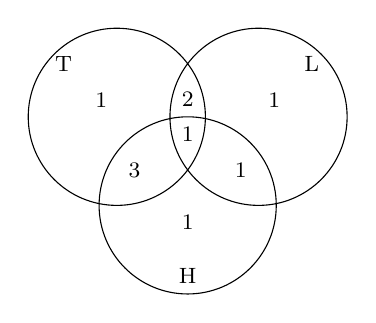
\begin{tikzpicture}[>=stealth,line join=round,line cap=round,font=\footnotesize,scale=0.45]
				\draw (0,0)node[above left]{$1$}circle (2.5) (4,0)node[above right]{$1$}circle(2.5) (2,-2.5)node[below]{$1$}circle(2.5);
				\draw (2,-0.5)node{$1$} (2,0.5)node{$2$} (0.5,-1.5)node{$3$} (3.5,-1.5)node{$1$} (-1.5,1.5)node{T} (5.5,1.5)node{L} (2,-4.5)node{H};
			\end{tikzpicture}}}
\end{ex}

\begin{ex}%[Pj31--2-Đề KT Theo Bài--TeamTeXHoa--Phan Anh]%[0D1H3-5]
	Trong kì thi học sinh giỏi cấp trường, lớp 11B có $15$ học sinh giỏi Văn, $22$ học sinh giỏi Toán. Tìm số học sinh giỏi cả Văn và Toán biết lớp đó có $40$ học sinh, và có $14$ học sinh không đạt học sinh giỏi.
	\choice
	{$4$}
	{$7$}
	{\True $11$}
	{$20$}
	\loigiai{Số học sinh học giỏi ít nhất một trong hai môn Toán và Văn là $40-14=26$.\\
		Số học sinh chỉ giỏi Toán mà không giỏi Văn
		là $26-15=11$.\\
		Vậy số học sinh giỏi cả hai môn Toán và Văn là $22-11=11$.\\
		\textbf{Cách khác:}
		Số học sinh học giỏi ít nhất một trong hai môn Toán và Văn là $40-14=26$.\\
		Số học sinh giỏi cả hai môn Toán và Văn là $22+15-26=11$.}
\end{ex}
\Closesolutionfile{ans}
\TNTF
\setcounter{ex}{0}
\Opensolutionfile{ans}[ans/ansDS-0D1-OnChuong-De1]
\begin{ex}%[Pj31--2-Đề KT Theo Bài--TeamTeXHoa--Phan Anh]%[0D1H1-4]
	Cho biết tính đúng sai của mỗi mệnh đề sau.
	\choiceTF
	{Nếu số $a$ chia hết cho $3$ thì $a$ chia hết cho $6$}
	{\True Nếu $\triangle ABC$ cân tại $A$ thì $\triangle ABC$ có $AB=AC$}
	{\True Tứ giác $ABCD$ là hình vuông khi và chỉ khi $ABCD$ là hình chữ nhật và có $AC$ vuông góc với $BD$}
	{$\pi^2>10$}
	\loigiai{\begin{itemchoice}
			\itemch \lq\lq Nếu số $a$ chia hết cho $3$ thì $a$ chia hết cho $6$\rq\rq  là mệnh đề sai vì nếu xét $a=3$ thì $a$ chia hết cho $3$ nhưng không chia hết cho $6$.
			\itemch \lq\lq Nếu $\triangle ABC$ cân tại $A$ thì $\triangle ABC$ có $AB=AC$\rq\rq  là mệnh đề đúng.
			\itemch \lq\lq Tứ giác $ABCD$ là hình vuông khi và chỉ khi $ABCD$ là hình chữ nhật và có $AC$ vuông góc với $BD$\rq\rq  là mệnh đề đúng.
			\itemch \lq\lq $\pi^2>10$\rq\rq  là mệnh đề sai, vì $\pi^2\approx9{,}869<10$.
		\end{itemchoice}}
\end{ex}

\begin{ex}%[Pj31--2-Đề KT Theo Bài--TeamTeXHoa--Phan Anh]%[0D1H1-2]
	Cho biết mệnh đề phủ định của mệnh đề sau đúng hay sai?
	\choiceTF
	{$P\colon$ \lq\lq Hình thoi có hai đường chéo vuông góc với nhau \rq\rq }
	{$S\colon$ \lq\lq $1>-3$ \rq\rq }
	{\True $K\colon$ \lq\lq Phương trình $x^4-2x^2+2=0$ có nghiệm \rq\rq }
	{$H\colon$ \lq\rq $\left(\sqrt{3}-\sqrt{12}\right)^2=3$ \rq\rq}
	\loigiai{
		\begin{itemchoice}
			\itemch Ta có mệnh đề phủ định là $\overline{P}\colon$ \lq\lq Hình thoi có hai đường chéo không vuông góc với nhau\rq\rq~ là mệnh đề sai.
			\itemch Ta có mệnh đề phủ định là $\overline{S}\colon$ \lq\lq $1\le-3$\rq\rq~ là mệnh đề sai.
			\itemch Ta có mệnh đề phủ định là $\overline{K}\colon$ \lq\lq phương trình $x^4-2x^2+2=0$ vô nghiệm\rq\rq~ là mệnh đề đúng. 
			\itemch Ta có mệnh đề phủ định là: $\overline{H}\colon$ \lq\lq $\left(\sqrt{3}-\sqrt{12}\right)^2\ne 3$\rq\rq~ là mệnh đề sai.
		\end{itemchoice}}
\end{ex}

\begin{ex}%[Pj31--2-Đề KT Theo Bài--TeamTeXHoa--Phan Anh]%[0D1H3-1]
	Cho các tập hợp $A=\{-3;-2;-1;0;1;2;3\}$; $B=\{0;1;4;5\}$; $C=\{-4;-3;1;2;5;6\}$. Khi đó
	\choiceTF
	{\True $A\cup B=\{-3;-2;-1;0;1;2;3;4;5\}$}
	{$A\cap B=\{0\}$}
	{\True $(A\cup B)\cap C=\{-3;1;2;5\}$}
	{\True $A\cap B\cap C=\{1\}$}
	\loigiai{
		\begin{itemchoice}
			\itemch $A\cup B=\{-3;-2;-1;0;1;2;3;4;5\}$.
			\itemch $A\cap B=\{0;1\}$.
			\itemch $(A\cup B)\cap C=\{-3;1;2;5\}$.
			\itemch $A\cap B\cap C=\{1\}$.
		\end{itemchoice}
		}
\end{ex}

\begin{ex}%[Pj31--2-Đề KT Theo Bài--TeamTeXHoa--Phan Anh]%[0D1H3-5]
	Lớp 10A có tất cả $50$ học sinh trong đó có $13$ học sinh chỉ thích đá bóng, $18$ học sinh chỉ thích chơi cầu lông, $10$ học sinh không thích môn nào trong hai môn thể thao nói trên và số học sinh còn lại thích chơi cả hai môn thể thao nói trên. Khi đó
	\choiceTF
	{\True Có $40$ học sinh thích chơi môn cầu lông hoặc môn bóng đá}
	{Có $27$ học sinh thích chơi cả hai môn cầu lông và bóng đá}
	{\True Có $31$ học sinh thích chỉ một trong hai môn bóng đá và môn cầu lông}
	{Có $26$ học sinh thích cầu lông}
	\loigiai{
		\begin{itemchoice}
			\itemch Số học sinh thích chơi môn cầu lông hoặc môn bóng đá là $50-10=40$ (học sinh).
			\itemch Số học sinh thích chơi cả hai môn câu lông và bóng đá là $40-(18+13)=9$ (học sinh).
			\itemch Số học sinh thích chỉ một trong hai môn bóng đá và môn cầu lông là $40-9=31$ (học sinh).
			\itemch Số học sinh thích câu lông là $18+9=27$ (học sinh).
		\end{itemchoice}
		}
\end{ex}
\Closesolutionfile{ans}
\TNSA
\setcounter{ex}{0}
\Opensolutionfile{ans}[ans/ansTLN-0D1-OnChuong-De1]

\begin{ex}%[Pj31--2-Đề KT Theo Bài--TeamTeXHoa--Phan Anh]%[0D1H1-3]
	Cho $x\in\mathbb{Z}$, xét hai mệnh đề chứa biến $A\colon\lq\lq x\ge3$\rq\rq  và $B\colon\lq\lq x\le a$\rq\rq . Để mệnh đề $B$ là phủ định của mệnh đề $A$ thì giá trị của $a$ là bao nhiêu?
	\shortans[oly]{2}
	\loigiai{
		Mệnh đề phủ định của $A$ là $\overline{A}\colon\lq\lq x<3$\rq\rq .\\
		Do $x\in\mathbb{Z}$ nên $\overline{A}\colon\lq\lq x\le2$\rq\rq .\\
		Do đó để mệnh đề $B$ là phủ định của mệnh đề $A$ thì $a=2$.
	}
\end{ex}
\begin{ex}%[Pj31--2-Đề KT Theo Bài--TeamTeXHoa--Phan Anh]%[0D1H1-2]
	Có bao nhiêu giá trị của $n\in\mathbb{N}$, $n\in(1;30)$ để mệnh đề $A\colon$\lq\lq Nếu $2n^2+3n+1$ chia hết cho $2$ thì $n$ chia hết cho $3$\rq\rq  là mệnh đề sai?
	\shortans[oly]{10}
	\loigiai{
		Mệnh đề $P\Rightarrow Q$ sai khi và chỉ khi $P$ đúng, $Q$ sai.\\
		Mệnh đề $P$ đúng khi $2n^2+3n+1=(2n+1)(n+1)$ chia hết cho $2$.\\
		Do $2n+1$ là số lẻ nên $n+1$ là số chẵn, suy ra $n$ là số lẻ.\\
		Mệnh đề $Q$ sai khi $Q$ không chia hết cho $3$.\\
		Vì $n\in(1;30)$ có $10$ số lẻ và không chia hết cho $3$ nên $n\in\{1;5;7;11;13;17;19;23;25;29\}$, vậy ta có $10$ giá trị $n$ thoả mãn bài toán.
		}
\end{ex}
\begin{ex}%[Pj31--2-Đề KT Theo Bài--TeamTeXHoa--Phan Anh]%[0D1V3-3]
	Cho hai tập hợp $A=[m-3;m+2]$, $B=(-3;5)$ với $m\in\mathbb{R}$. Tính tổng tất cả các giá trị nguyên của $m$ để $A\cap B$ khác tập rỗng.
	\shortans[oly]{18}
	\loigiai{
		Trước hết, ta tìm $m$ để $A\cap B=\varnothing$.\\
		Để $A\cap B=\varnothing$ thì $\hoac{&m+2\le-3\\&m-3\ge5}\Leftrightarrow\hoac{&m\le-5\\&m\ge8.}$.\\
		Vậy để $A\cap B$ khác tập rỗng thì $-5<m<8$.\\
		Do $m$ nguyên nên $m\in\{-4;-3;-2;-1;0;1;2;3;4;5;6;7\}$, suy ra tổng các giá trị của $m$ là
		\[S=-4-3-2-1+1+0+1+2+3+4+5+6+7=18.\]
		}
\end{ex}

\begin{ex}%[Pj31--2-Đề KT Theo Bài--TeamTeXHoa--Phan Anh]%[0D1H2-2]
	Cho tập hợp $B=\left\{x\in\mathbb{Z}\mid\left|x^2+1\right|\le2\right\}$. Tập hợp $B$ có bao nhiêu tập con gồm $2$ phần tử?
	\shortans[oly]{3}
	\loigiai{
		Ta có: $\heva{&x\in\mathbb{Z}\\&\left|x^2+1\right|\le2}\Rightarrow\hoac{&x=-1\\&x=0\\&x=1}\Rightarrow B=\{-1;0;1\}$.\\
		Các tập con của tập $B$ gồm $2$ phần tử là $\{-1;0\},\{0;1\},\{-1;1\}$.\\
		Vậy có $3$ tập con của $B$ gồm $2$ phần tử.
		}
\end{ex}

\begin{ex}%[Pj31--2-Đề KT Theo Bài--TeamTeXHoa--Phan Anh]%[0D1H3-5]
	Bạn A Súa thống kê số ngày có mưa, có sương mù ở bản mình trong tháng $3$ vào một thời điểm nhất định và được kết quả như sau: $14$ ngày có mưa, $15$ ngày có sương mù, trong đó $10$ ngày có cả mưa và sương mù. Hỏi trong tháng $3$ đó có bao nhiêu ngày không có mưa và không có sương mù?
	\shortans[oly]{12}
	\loigiai{
		Gọi $A$, $B$ lần lượt là tập hợp các ngày có mưa, có sương mù. Khi đó, $A\cap B$ là tập hợp các ngày có cả mưa và sương mù, $A\cup B$ là tập hợp các ngày hoặc có mưa hoặc có sương mù.\\
		Ta có $n(A)=14$, $n(B)=15$, $n(A\cap B)=10$.\\
		Số ngày hoặc có mưa hoặc có sương mù là
		\[n(A\cup B)=n(A)+n(B)-n(A\cap B)=14+15-10=19\text{ (ngày).}\]
		Tháng $3$ có $31$ ngày nên số ngày không có mưa và không có sương mù trong tháng $3$ đó là $31-19=12$ (ngày).
		}
\end{ex}

\begin{ex}%[Pj31--2-Đề KT Theo Bài--TeamTeXHoa--Phan Anh]%[0D1V3-5]
	Trong đợt khảo sát nghề, giáo viên chủ nhiệm lớp 10D đưa ra ba nhóm ngành cho học sinh lựa chọn, đó là: Giáo dục, Y tế, Công nghệ thông tin. Học sinh có thể chọn từ một đến ba nhóm ngành nêu trên hoặc không chọn nhóm ngành nào trong ba nhóm ngành trên. Giáo viên chủ nhiệm thống kê theo từng nhóm ngành và được kết quả: có $6$ học sinh chọn nhóm ngành Giáo dục, $9$ học sinh chọn nhóm ngành Y tế, $10$ học sinh chọn nhóm ngành Công nghệ thông tin, $22$ học sinh không chọn nhóm ngành nào trong ba nhóm trên. Nếu thống kê số lượng học sinh chọn theo từng hai nhóm ngành được kết quả: có $3$ học sinh chọn hai nhóm ngành Giáo dục và Y tế, $2$ học sinh chọn hai nhóm ngành Y tế và Công nghệ thông tin, $3$ học sinh chọn hai nhóm ngành Giáo dục và Công nghệ thông tin. Hỏi có bao nhiêu học sinh chọn cả ba nhóm ngành nêu trên biết lớp 10D có $40$ học sinh?
	\shortans[oly]{1}
	\loigiai{
		Gọi $A$, $B$, $C$ lần lượt là tập hợp học sinh chọn nhóm ngành Giáo dục, Y tế, Công nghệ thông tin.\\
		Khi đó, $A\cup B\cup C$ là tập hợp các học sinh chọn ít nhất một trong ba nhóm ngành trên.\\
		Do lớp 10D có $40$ học sinh và $22$ học sinh không chọn nhóm ngành trong ba nhóm ngành trên nên số học sinh chọn ít nhất một trong ba nhóm ngành trên là $40-22=18$.\\
		Ta có $n(A)=6$, $n(B)=9$, $n(C)=10$, $n(A\cup B\cup C)=18$, $n(A\cap B)=3$, $n(B\cap C)=2$, $n(A\cap C)=3$.\\
		Ta có số học sinh chọn cả ba nhóm ngành nêu trên là
		\begin{eqnarray*}
			n(A\cap B\cap C)&=&n(A\cup B\cup C)+n(A\cap B)+n(B\cap C)+n(A\cap C)-n(A)-n(B)-n(C)\\
			&=&18+3+2+3-6-9-10=1.
		\end{eqnarray*}
		}
\end{ex}
\Closesolutionfile{ans}
% \begin{center}	
% 	\fontfamily{qag}\selectfont\color{violet} 	\centering{\textbf{BẢNG ĐÁP ÁN}}
% \end{center}
% \inputansbox{12}{ans/ansBONPA-0D1-OnChuong-De1}
% \inputansbox{4}{ans/ansDS-0D1-OnChuong-De1}
% \inputansbox{6}{ans/ansTLN-0D1-OnChuong-De1}